\begin{figure}[h]
  \centering
  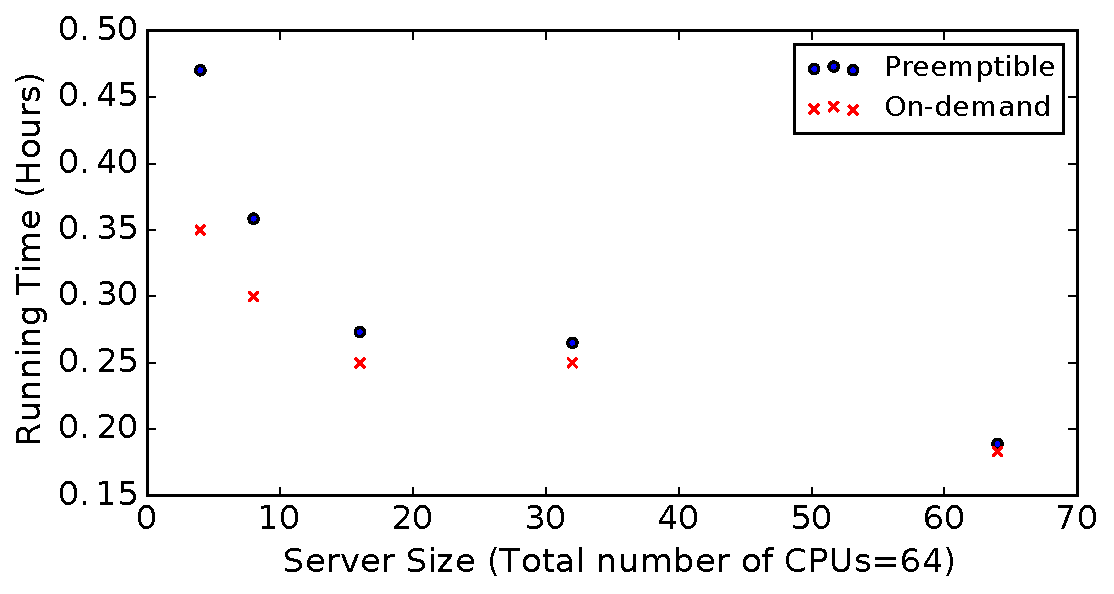
\includegraphics[width=0.4\textwidth]{../graphs/confin_64_time.pdf}
  \caption{confinement running times}
  \label{fig:confin-64-times}
\end{figure}


\begin{figure}[h]
  \centering
  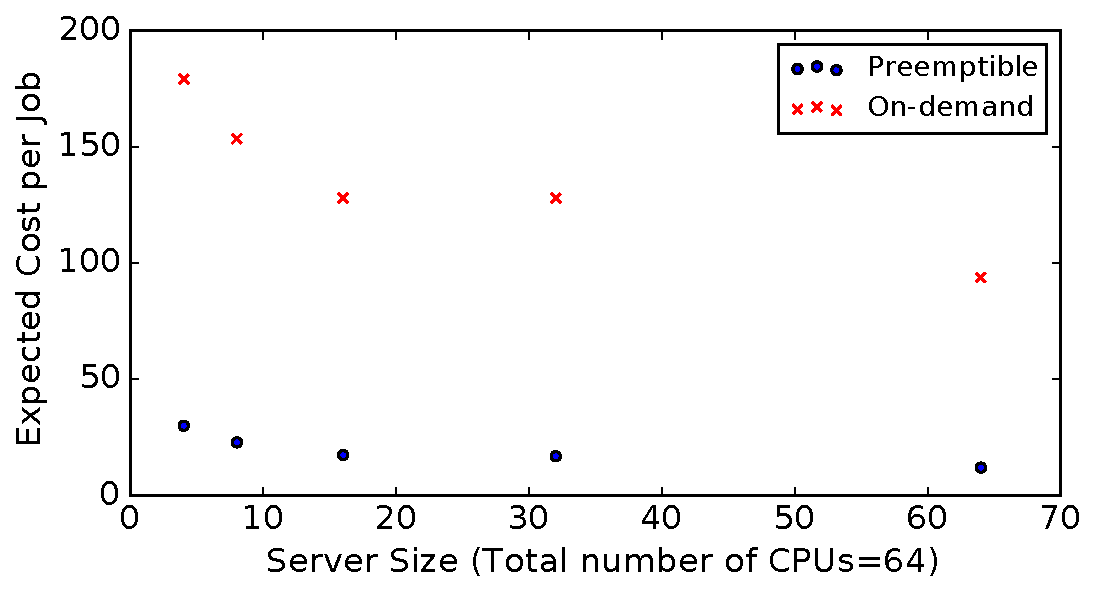
\includegraphics[width=0.4\textwidth]{../graphs/confin_64_cost.pdf}
  \caption{confinement cost}
  \label{fig:confin-64-cost}
\end{figure}



\begin{figure}[h]
  \centering
  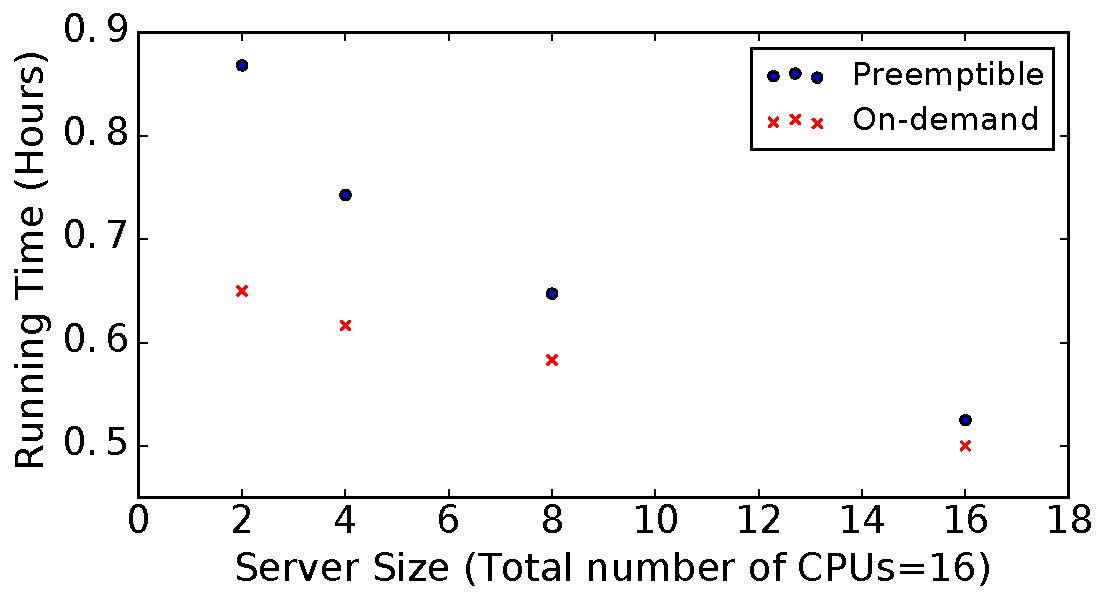
\includegraphics[width=0.4\textwidth]{../graphs/confin_16_time.pdf}
  \caption{confinement running times}
  \label{fig:confin-16-times}
\end{figure}


\begin{figure}[h]
  \centering
  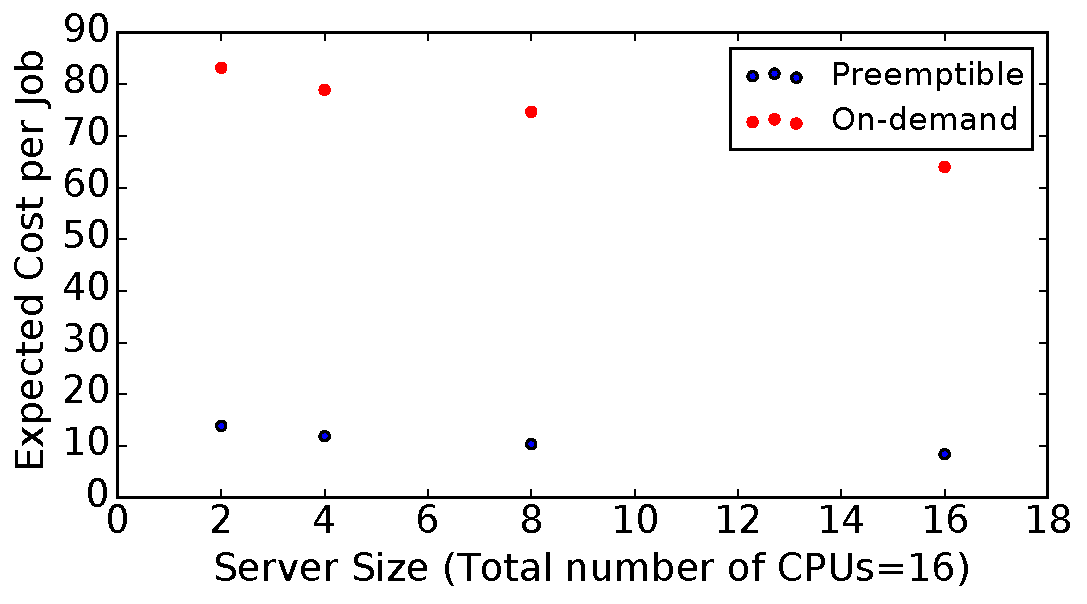
\includegraphics[width=0.4\textwidth]{../graphs/confin_16_cost.pdf}
  \caption{confinement cost}
  \label{fig:confin-16-cost}
\end{figure}



\begin{figure}
  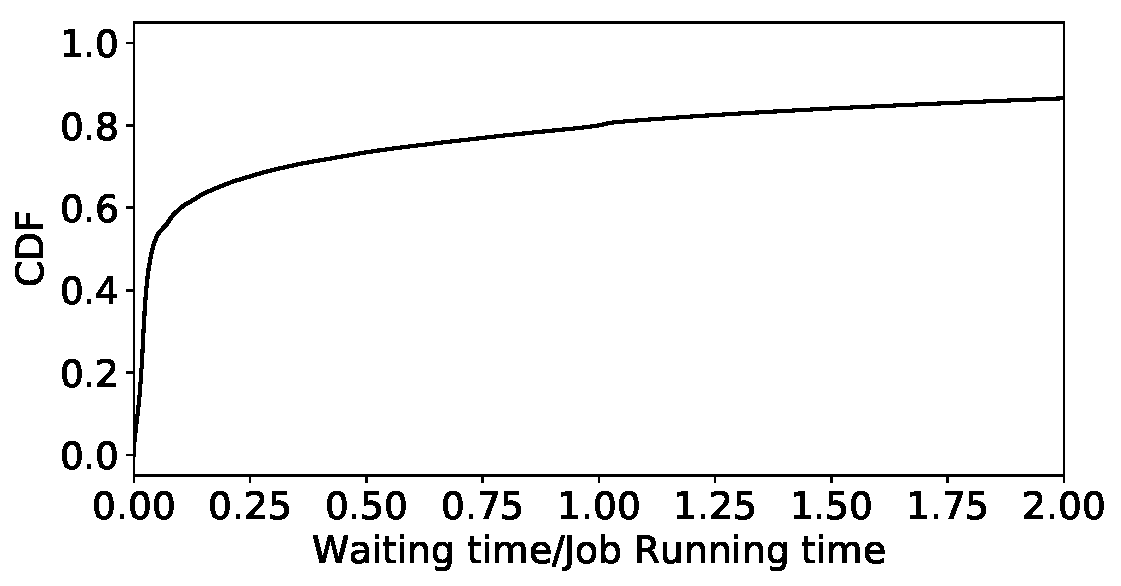
\includegraphics[width=0.4\textwidth]{../data/waiting_all.pdf}
  \caption{Ratio of waiting time to job running time on an HPC cluster. Average is 0.2}
  \label{fig:hpc-wait-cdf}
\end{figure}


\begin{figure}
  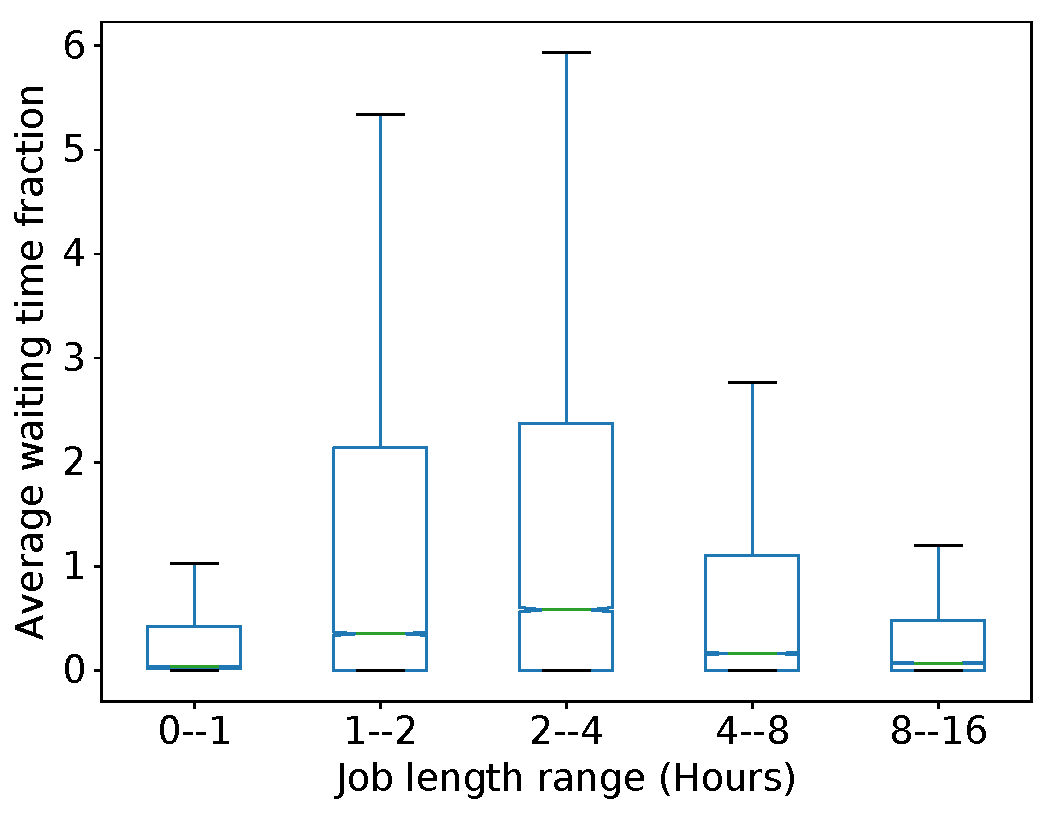
\includegraphics[width=0.4\textwidth]{../graphs/waiting_time_buckets.pdf}
  \caption{Waiting time fraction of jobs of different lengths varies.}
  \label{fig:hpc-wait-buckets}  
\end{figure}



%%% Local Variables:
%%% mode: latex
%%% TeX-master: "paper"
%%% End:
